\section{Usability Principles}
Much progress has been made in the design of application, such that users enjoy using a site and are therefore more likely to recommend it and to reuse the site. David Benyon composed usability principles which act as a guideline when designing applications with the users in mind. These principles aim to improve consistency, familiarity and intuitiveness of applications.

The screenshots in figure \ref{fig:Twitter_Changes} highlight how the design of websites have changed. In particular, the design in image \ref{fig:Twitter_2017} shows how Twitter now use a more simplistic flat design, which uses bright colours so key areas of the page a clearly visible and separated. This is as opposed to the design in \ref{fig:Twitter_2006}, which uses a lot of gradients. This draws attention away from the important features in the site and makes it appear more cluttered. This shows how the designs have been adapted in order to make them more usable. Fidelis will also aim to make the application more usable through the use of design principles, as discussed in this section.

\begin{figure}[H]
	\centering
	\begin{subfigure}[t]{0.45\textwidth}
		\centering
		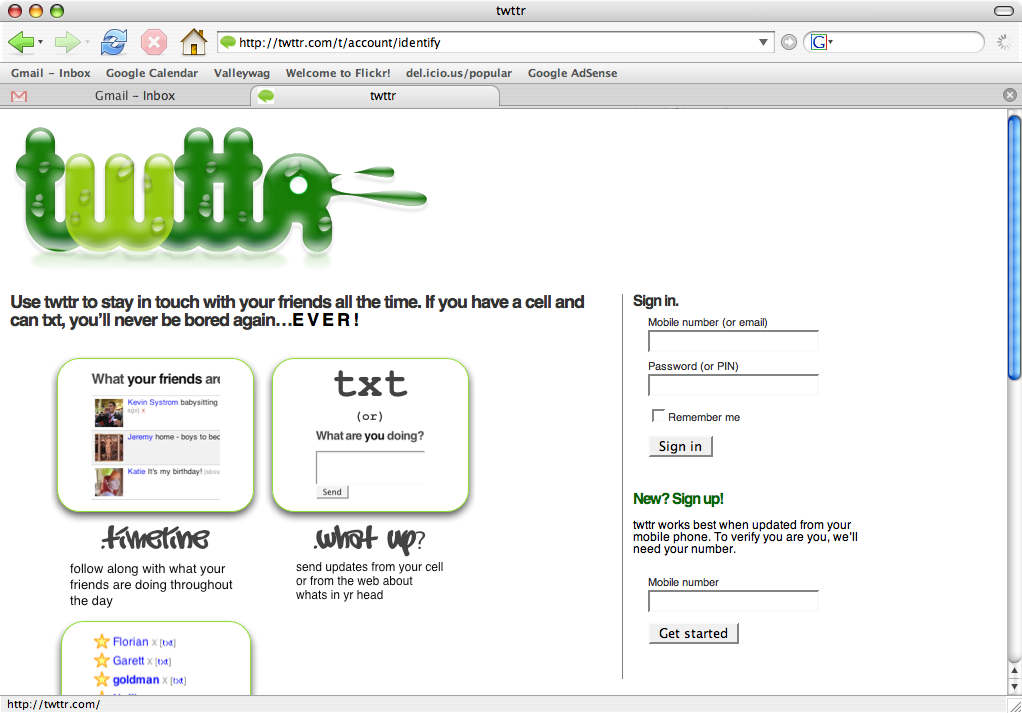
\includegraphics[width=1.0\textwidth, height=125px]{Images/Design/Twitter_2006}
		\caption{Twitter in 2006}\label{fig:Twitter_2006}		
	\end{subfigure}
	\quad
	\begin{subfigure}[t]{0.45\textwidth}
		\centering
		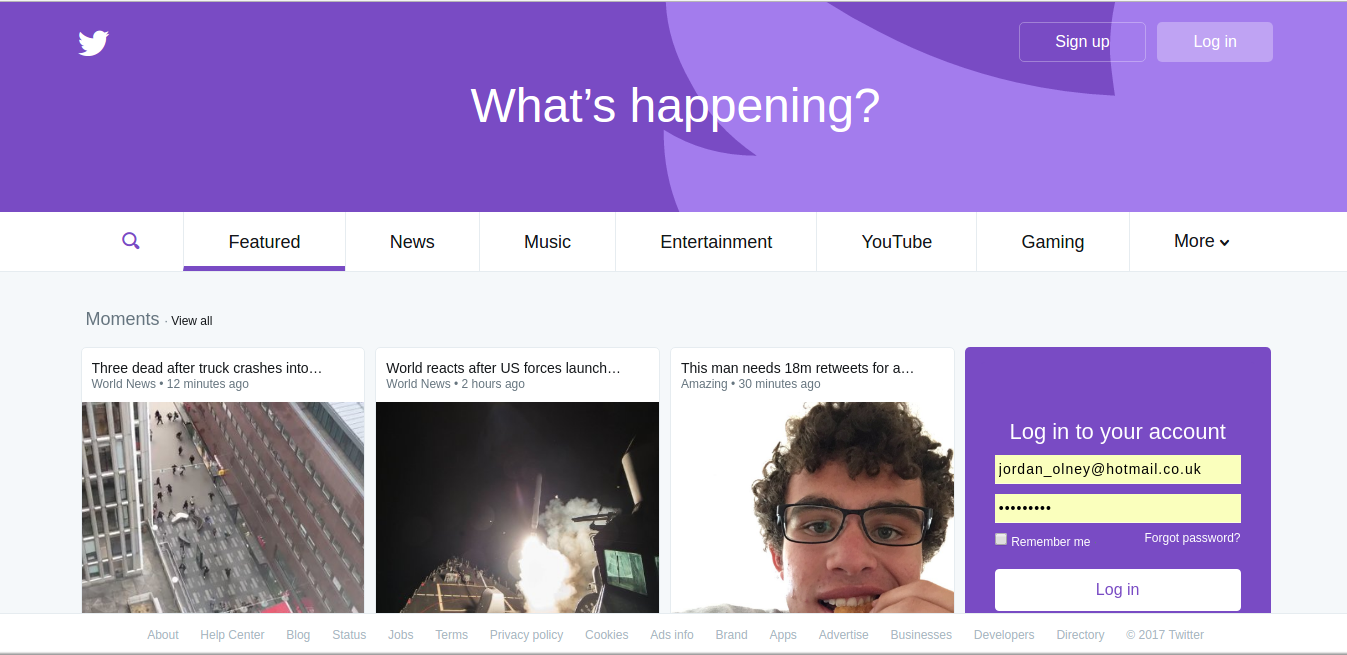
\includegraphics[width=1.0\textwidth, height=125px]{Images/Design/Twitter_2017}
		\caption{Twitter in 2017}\label{fig:Twitter_2017}
	\end{subfigure}
	\caption{Twitter in 2006 and 2017}\label{fig:Twitter_Changes}
\end{figure}

\subsection{Consistency}

\subsection{Familiarity}
Discuss move from old gradients to now flat designs which people are familiar with

\subsection{Intuitive Design}